\documentclass[12pt]{article}
%%%%%%%%%%%%%%%%
% Packages
%%%%%%%%%%%%%%%%

\usepackage[top=1.5cm,bottom=1.5cm,left=1.5cm,right= 1.5cm]{geometry}
\usepackage[parfill]{parskip}
\usepackage{graphicx, fontspec, xcolor,multicol, enumitem, setspace, amsmath, changepage}
\DeclareGraphicsRule{.tif}{png}{.png}{`convert #1 `dirname #1`/`basename #1 .tif`.png}

%%%%%%%%%%%%%%%%
% User defined colors
%%%%%%%%%%%%%%%%

% Pantone 2015 Fall colors
% http://iwork3.us/2015/02/18/pantone-2015-fall-fashion-report/
% update each semester or year

\xdefinecolor{custom_blue}{rgb}{0, 0.32, 0.48} % FROM SPRING 2016 COLOR PREVIEW
\xdefinecolor{custom_darkBlue}{rgb}{0.20, 0.20, 0.39} % Reflecting Pond  
\xdefinecolor{custom_orange}{rgb}{0.96, 0.57, 0.42} % Cadmium Orange
\xdefinecolor{custom_green}{rgb}{0, 0.47, 0.52} % Biscay Bay
\xdefinecolor{custom_red}{rgb}{0.58, 0.32, 0.32} % Marsala

\xdefinecolor{custom_lightGray}{rgb}{0.78, 0.80, 0.80} % Glacier Gray
\xdefinecolor{custom_darkGray}{rgb}{0.35, 0.39, 0.43} % Stormy Weather

%%%%%%%%%%%%%%%%
% Color text commands
%%%%%%%%%%%%%%%%

%orange
\newcommand{\orange}[1]{\textit{\textcolor{custom_orange}{#1}}}

% yellow
\newcommand{\yellow}[1]{\textit{\textcolor{yellow}{#1}}}

% blue
\newcommand{\blue}[1]{\textit{\textcolor{blue}{#1}}}

% green
\newcommand{\green}[1]{\textit{\textcolor{custom_green}{#1}}}

% red
\newcommand{\red}[1]{\textit{\textcolor{custom_red}{#1}}}

%%%%%%%%%%%%%%%%
% Coloring titles, links, etc.
%%%%%%%%%%%%%%%%

\usepackage{titlesec}
\titleformat{\section}
{\color{custom_blue}\normalfont\Large\bfseries}
{\color{custom_blue}\thesection}{1em}{}
\titleformat{\subsection}
{\color{custom_blue}\normalfont}
{\color{custom_blue}\thesubsection}{1em}{}

\newcommand{\ttl}[1]{ \textsc{{\LARGE \textbf{{\color{custom_blue} #1} } }}}

\newcommand{\tl}[1]{ \textsc{{\large \textbf{{\color{custom_blue} #1} } }}}

\usepackage[colorlinks=false,pdfborder={0 0 0},urlcolor= custom_orange,colorlinks=true,linkcolor= custom_orange, citecolor= custom_orange,backref=true]{hyperref}

%%%%%%%%%%%%%%%%
% Instructions box
%%%%%%%%%%%%%%%%

\newcommand{\inst}[1]{
\colorbox{custom_blue!20!white!50}{\parbox{\textwidth}{
	\vskip10pt
	\leftskip10pt \rightskip10pt
	#1
	\vskip10pt
}}
\vskip10pt
}
\usepackage{fancyvrb}	% for colored code chunks
\usepackage{lscape}

%%%%%%%%%%%
% App Ex number    %
%%%%%%%%%%%

% DON'T FORGET TO UPDATE

\newcommand{\appno}[1]
{7.1}

%%%%%%%%%%%%%%
% Turn on/off solutions       %
%%%%%%%%%%%%%%
%:

% Off
\newcommand{\soln}[2]{$\:$\\ \vspace{#1}}{}

% On
%\newcommand{\soln}[2]{\textit{\textcolor{custom_red}{#2}}}{}

%%%%%%%%%%%%%%%%
% Document
%%%%%%%%%%%%%%%%

\begin{document}
\fontspec[Ligatures=TeX]{Helvetica Neue Light}

Dr. \c{C}etinkaya-Rundel \hfill Sta 101: Data Analysis and Statistical Inference \\
Duke University - Department of Statistical Science \hfill \\

\ttl{Application exercise \appno{}: \\
Multiple linear regression}

\inst{$\:$ \\
Team name: \rule{10cm}{0.5pt} \\
$\:$ \\
Lab section: $\qquad$ 8:30 $\qquad$ 10:05 $\qquad$ 11:45 $\qquad$ 1:25 $\qquad$ 3:05 $\qquad$ 4:40 \\
$\:$ \\
Write your responses in the spaces provided below. WRITE LEGIBLY and SHOW ALL WORK! 
Only one submission per team is required. One team will be randomly selected and their 
responses will be discussed and graded. Concise and coherent are best!}

%%%%%%%%%%%%%%%%%%%%%%%%%%%%%%%%%%%%

\section*{Cigarettes and CO}

The Federal Trade Commission annually rates varieties of domestic cigarettes according to their tar, nicotine, and carbon monoxide content. The United States Surgeon General considers each of these substances hazardous to a smoker's health. Past studies have shown that increases in the tar and nicotine content of a cigarette are accompanied by an increase in the carbon monoxide emitted from the cigarette smoke.

In this exercise we will work with data from 2007 on cigarettes sold in the US. Each row in the dataset represents a cigarette. There are 11 variables in the dataset:
{\small
\begin{itemize}
\item \texttt{BRAND\_NAME}
\item \texttt{TYPE}: Type of cigarette, REGULAR or MENTHOL
\item \texttt{NIC}: Nicotine content, in mg
\item \texttt{TAR}: Tar content, in mg
\item \texttt{CO}: Carbon monoxide, in mg
\item \texttt{LEN}: Length of cigarette, in mm
\item \texttt{FLTR}: Filter, F or NF
\item \texttt{PACK}: Pack type, HARD or SOFT   
\item \texttt{STRENGTH}: Strength of cigarette, ULTRA LIGHT, LIGHT, MEDIUM, REGULAR FULL, or FLAVOR
\item \texttt{STYLE}: Some information of style of cigarette (not available for all cigarettes, and not used in this analysis)
\item \texttt{OTHER}: Other relevant information (not available for all cigarettes, and not used in this analysis)
\end{itemize}
}

$\:$ 

\begin{enumerate}

\item Suppose the full model uses the following explanatory variables: nicotine, tar, length, filter, pack, strength, and type.
Describe, briefly, in your own words, how you would carry out model selection using the backwards elimination method based on adjusted $R^2$.

\soln{2cm}{
Fit full model, record its adjusted $R^2$. Then, drop one variable at a time, record each model's adjusted $R^2$. Then, move to the
model with the highest adjusted $R^2$. Stop when adjusted $R^2$ stops increasing.
}

% 

\item The output of the model resulting from backwards elimination with adjusted $R^2$ is shown below. Evaluate the slopes of NIC and 
TAR variables. Are these results surprising? Why, or why not? Make sure to use appropriate terminology in your answer. \textit{Hint:} The 
pairs plot will at the end of this document can be helpful for determining whether the results are surprising or not.

\begin{minipage}[c]{0.55\textwidth}
{\footnotesize
\begin{tabular}{rrrrr}
  \hline
 & Estimate & Std. Error & t value & Pr($>$$|$t$|$) \\ 
  \hline
(Intercept) & -0.5489 & 0.5395 & -1.02 & 0.3092 \\ 
  NIC & -4.0406 & 0.4342 & -9.31 & 0.0000 \\ 
  TAR & 1.0485 & 0.0441 & 23.80 & 0.0000 \\ 
  LEN & 0.0350 & 0.0055 & 6.38 & 0.0000 \\ 
  FLTRNF & -6.4925 & 0.3577 & -18.15 & 0.0000 \\ 
  PACKSOFT & 0.5128 & 0.1046 & 4.90 & 0.0000 \\ 
  STRENGTHLIGHT & 1.6804 & 0.2110 & 7.96 & 0.0000 \\ 
  STRENGTHMEDIUM & 0.7339 & 0.4607 & 1.59 & 0.1114 \\ 
  STRENGTHREGULAR & 0.2801 & 0.3059 & 0.92 & 0.3600 \\ 
  STRENGTHFULL FLAVOR & 2.2447 & 0.3287 & 6.83 & 0.0000 \\ 
   \hline
\end{tabular}
}
\end{minipage}
\begin{minipage}[c]{0.4\textwidth}
$\:$ \\
\end{minipage}

\soln{3cm}{
Yes, according to this model output, as nicotine increases CO emission decreases. But we know from the pairs plot that nicotine and CO are
positively associated. This is likely due to multicollinearity in the model -- nicotine and tar are strongly correlated, resulting in unreliable
slope estimates.
}

$\:$

%

\item Next, we try the following two models, and obtain the following adjusted $R^2$ values:
\begin{itemize}
\item Option 1, remove TAR: \texttt{lm(CO $\sim$ NIC + LEN + FLTR + PACK + STRENGTH, data = cig07)}, \\
adjusted $R^2$ = 0.7066
\item Option 2, remove NIC: \texttt{lm(CO $\sim$ TAR + LEN + FLTR + PACK + STRENGTH, data = cig07)}, \\
adjusted $R^2$ = 0.7857
\end{itemize}
Based on these results which variable should we keep in our full model, nicotine or tar? Why?

\soln{1cm}{Remove nicotine, higher adjusted $R^2$.}

%

\pagebreak

\item In the remainder of the application exercise we will complete some inferential tasks based on the
final model. Use the following plots to check conditions before to determine whether we can proceed with these tasks.

\end{enumerate}

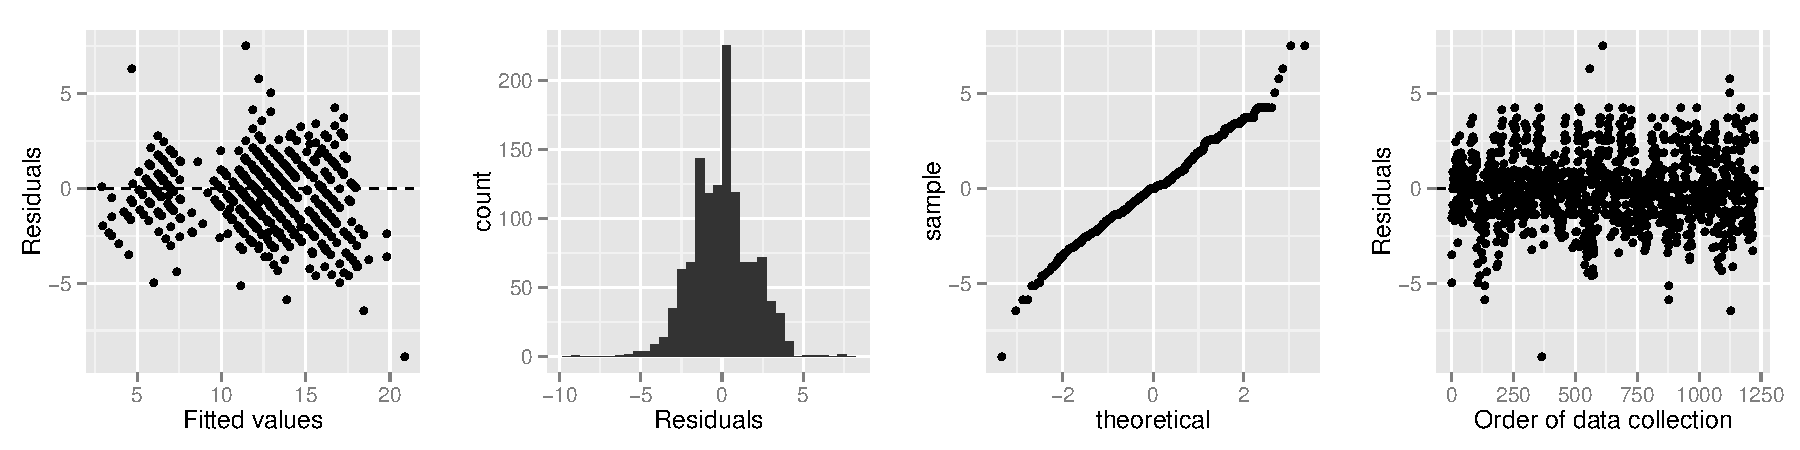
\includegraphics[width=\textwidth]{diag.pdf}

\soln{4cm}{
\begin{enumerate}
\item Linearity -- residuals scattered around 0, but there is some structure, may not be met.
\item Nearly normal residuals -- mostly met.
\item Constant variance -- residuals plot does not have an apparent fan shape.
\item Independence -- no apparent structure due to order of data collection, but we would like
to know about data collection methods (i.e. how were these cigarettes selected)
\end{enumerate}
}

%

\begin{enumerate}[resume]

\item Provided below is the final model output. Construct a 95\% confidence interval for the slope of 
the pack variable (PACKSOFT), and interpret it in context.

\begin{minipage}[c]{0.55\textwidth}
{\footnotesize
\begin{tabular}{rrrrr}
  \hline
 & Estimate & Std. Error & t value & Pr($>$$|$t$|$) \\ 
  \hline
(Intercept) & -0.0586 & 0.5555 & -0.11 & 0.9160 \\ 
  TAR & 0.7344 & 0.0293 & 25.07 & 0.0000 \\ 
  LEN & 0.0267 & 0.0056 & 4.76 & 0.0000 \\ 
  FLTRNF & -6.1949 & 0.3686 & -16.81 & 0.0000 \\ 
  PACKSOFT & 0.5597 & 0.1081 & 5.18 & 0.0000 \\ 
  STRENGTHLIGHT & 1.9077 & 0.2168 & 8.80 & 0.0000 \\ 
  STRENGTHMEDIUM & 0.7900 & 0.4766 & 1.66 & 0.0976 \\ 
  STRENGTHREGULAR & 0.5664 & 0.3149 & 1.80 & 0.0723 \\ 
  STRENGTHFULL FLAVOR & 3.0920 & 0.3268 & 9.46 & 0.0000 \\ 
   \hline
\end{tabular}
$\:$ \\
Residual standard error: 1.836 on 1216 degrees of freedom \\
Multiple R-squared:  0.7871,	Adjusted R-squared:  0.7857 \\
F-statistic: 561.8 on 8 and 1216 DF,  p-value: < 2.2e-16 \\
}
\end{minipage}
\begin{minipage}[c]{0.4\textwidth}
$\:$ \\
\end{minipage}

\soln{3cm}{
$df = 1216$, $t_{1216}^\star \approx 1.96$ \\
$0.5597 \pm 1.96 \times 0.1081 = (0.35, 0.77)$ \\
We are 95\% confident that, on average, soft pack cigarettes emit 0.35 mg to 0.77 mg more CO than hard pack cigarettes.
}

%

\pagebreak

\item The ANOVA output below shows the sum of squares attributed to each variable separately. Based on this output
which predictor is able to explain the highest portion of the variability in CO emission of cigarettes? What percent
of the variability in CO emission does this variable explain?

\begin{minipage}[c]{0.55\textwidth}
{\footnotesize
\begin{tabular}{lrrrrr}
  \hline
 & Df & Sum Sq & Mean Sq & F value & Pr($>$F) \\ 
  \hline
TAR & 1 & 12216.31 & 12216.31 & 3622.74 & 0.0000 \\ 
  LEN & 1 & 194.02 & 194.02 & 57.54 & 0.0000 \\ 
  FLTR & 1 & 1675.48 & 1675.48 & 496.86 & 0.0000 \\ 
  PACK & 1 & 169.17 & 169.17 & 50.17 & 0.0000 \\ 
  STRENGTH & 4 & 900.44 & 225.11 & 66.76 & 0.0000 \\ 
  Residuals & 1216 & 4100.50 & 3.37 &  &  \\ 
   \hline
\end{tabular}
}
\end{minipage}
\begin{minipage}[c]{0.4\textwidth}
$\:$ \\
\end{minipage}

\soln{3cm}{
$R^2_{TAR} = \frac{12216.31}{12216.31 + 194.02 + 1675.48 + 169.17 + 900.44 + 4100.50} \approx 0.63$
}

%

\item Using the regression model predict the CO emission for a cigarette with the following characteristics. Note that you 
may not need to use each attribute in your calculation.

\begin{multicols}{2}
\begin{itemize}
\item \texttt{BRAND\_NAME}: Sir Smokes-a-Lot
\item \texttt{TYPE}: MENTHOL
\item \texttt{NIC}: 0.75 mg
\item \texttt{TAR}: 12 mg
\item \texttt{LEN}: 80 mm
\item \texttt{FLTR}: F
\item \texttt{PACK}: HARD
\item \texttt{STRENGTH}: LIGHT
\end{itemize}
\end{multicols}

\soln{1.5cm}{
$\widehat{CO} = -0.0586 + 0.7344 * 12 + 0.0267 * 80 + 1.9077 = 12.79$
}

%

\item[Extra:] (If time permits) Load the data in R:

{\small
\begin{Verbatim}[frame=single, formatcom=\color{blue}]
load(url("https://stat.duke.edu/~mc301/data/cig07.RData"))
\end{Verbatim}
}

Now confirm your prediction from the previous question using the \texttt{predict} function in R. Note that your hand 
calculated prediction might be very slightly different from R's prediction, due to rounding of the coefficients on the regression output.
Also quantify the uncertainty around this prediction with a 95\% prediction interval.

{\small
\begin{Verbatim}[frame=single, formatcom=\color{blue}]
# fit the model
m = lm(CO ~ TAR + LEN + FLTR + PACK + STRENGTH, data = cig07)
# create the new data point
smokesalot = data.frame(TAR = 12, LEN = 80, FLTR = "F", PACK = "HARD", STRENGTH = "LIGHT")
# predict
predict(m, newdata = smokesalot, interval = "prediction")
\end{Verbatim}
}

\end{enumerate}

%%

\pagebreak

\begin{landscape}

\begin{center}
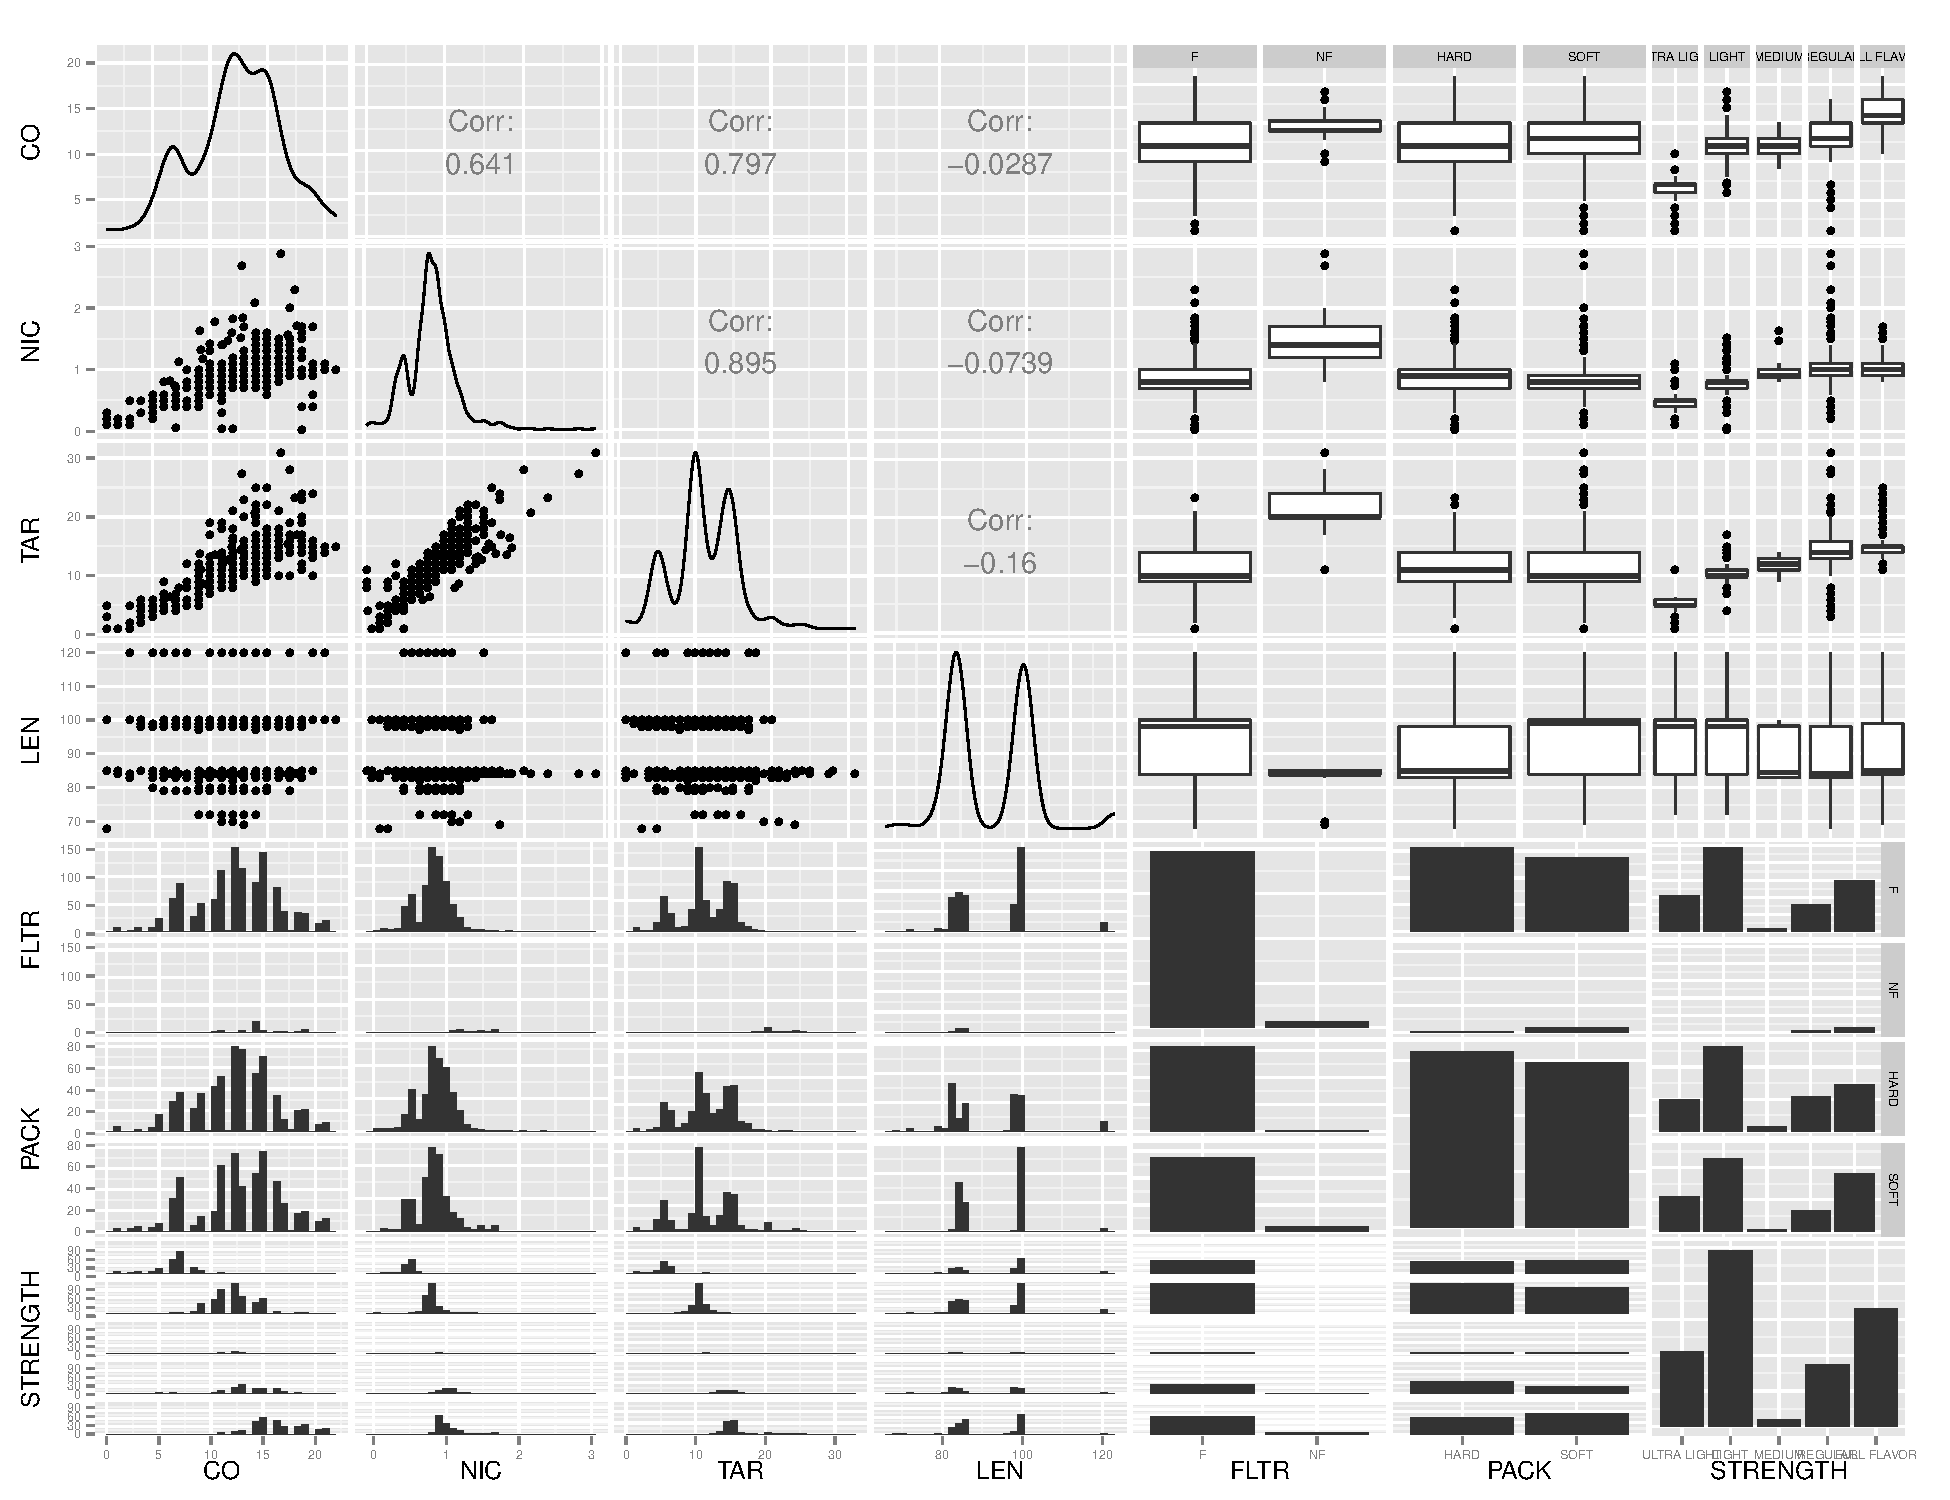
\includegraphics[width=1.2\textwidth]{pairs.pdf}
\end{center}

\end{landscape}

%


\end{document}